%\documentclass[final,hyperref={pdfpagelabels=false}]{beamer}
\documentclass[final]{beamer}
\usepackage{grffile}
\mode<presentation>{\usetheme{Icy}}
\usepackage[ngerman]{babel}
\usepackage[utf8]{inputenc}
\usepackage{amsmath,amsthm, amssymb, latexsym}
%\usepackage{times}\usefonttheme{professionalfonts}  % obsolete
%\usefonttheme[onlymath]{serif}
\boldmath
\usepackage[orientation=landscape,size=a0,scale=1.4,debug]{beamerposter}
% change list indention level
% \setdefaultleftmargin{3em}{}{}{}{}{}


%\usepackage{snapshot} % will write a .dep file with all dependencies, allows for easy bundling

\usepackage{array,booktabs,tabularx}
\newcolumntype{Z}{>{\centering\arraybackslash}X} % centered tabularx columns
\newcommand{\pphantom}{\textcolor{ta3aluminium}} % phantom introduces a vertical space in p formatted table columns??!!

\listfiles

\usepackage{tikz}
\usetikzlibrary{positioning,shapes}
\tikzstyle{rec}=[rectangle split, rectangle split parts =2, draw, 
  rounded corners, fill=i6colorscheme5,
minimum size=2em, minimum width=12em,text centered , text width = 12em, text centered]
\tikzstyle{comp}=[rec, fill=i6colorscheme1]


\newcommand{\cob}{Care-O-bot\textsuperscript{\textregistered}}

%%%%%%%%%%%%%%%%%%%%%%%%%%%%%%%%%%%%%%%%%%%%%%%%%%%%%%%%%%%%%%%%%%%%%%%%%%%%%%%%%%%%%%
\graphicspath{{figures/}}

\title{\huge Automatische Kalibrierung eines mobilen Roboterassistenten}
\author{Jannik Abbenseth}
\institute[Hochschule Furtwangen University]
{Fakultät für Maschinenbau und Verfahrenstechnik,
  Hochschule Furtwangen University
  \and
  Institut für Produktions- und Automatisierungstechnik,
  Fraunhofer Gesellschaft,
Stuttgart}
\date[20. Januar 2013]{20. Januar 2013}

%%%%%%%%%%%%%%%%%%%%%%%%%%%%%%%%%%%%%%%%%%%%%%%%%%%%%%%%%%%%%%%%%%%%%%%%%%%%%%%%%%%%%%
\newlength{\columnheight}
\setlength{\columnheight}{10cm}


%%%%%%%%%%%%%%%%%%%%%%%%%%%%%%%%%%%%%%%%%%%%%%%%%%%%%%%%%%%%%%%%%%%%%%%%%%%%%%%%%%%%%%
\begin{document}
\begin{frame}
  \begin{columns}[t]
    \begin{column}{.3\linewidth}

      %%%%%%%%%%%%%%%%%%%%%%%%%%%%%%%%%%%%%%%%%%%%%%%%%%%%%%%%%%%%%%%%%%%%%%%%%%%%%%%%%%%%%%%%%%%%%%%%%%%%%%%%%%%%

      \begin{block}{\phantom{fg}Der \cob}
        \begin{itemize}
          \item Serviceroboter für den Haushalt
            \begin{itemize}
              \item \alert {Interaktion} mit dem Menschen
              \item Wechselnde Umgebung
            \end{itemize}
          \item \alert{Roboterarm} mit sieben Freiheitsgraden
          \item \alert{Torso} mit drei bis vier Freiheitsgraden
          \item \alert{Stereo-} und \alert{3D Kameras} 
        \end{itemize}
        \vskip4.5ex
        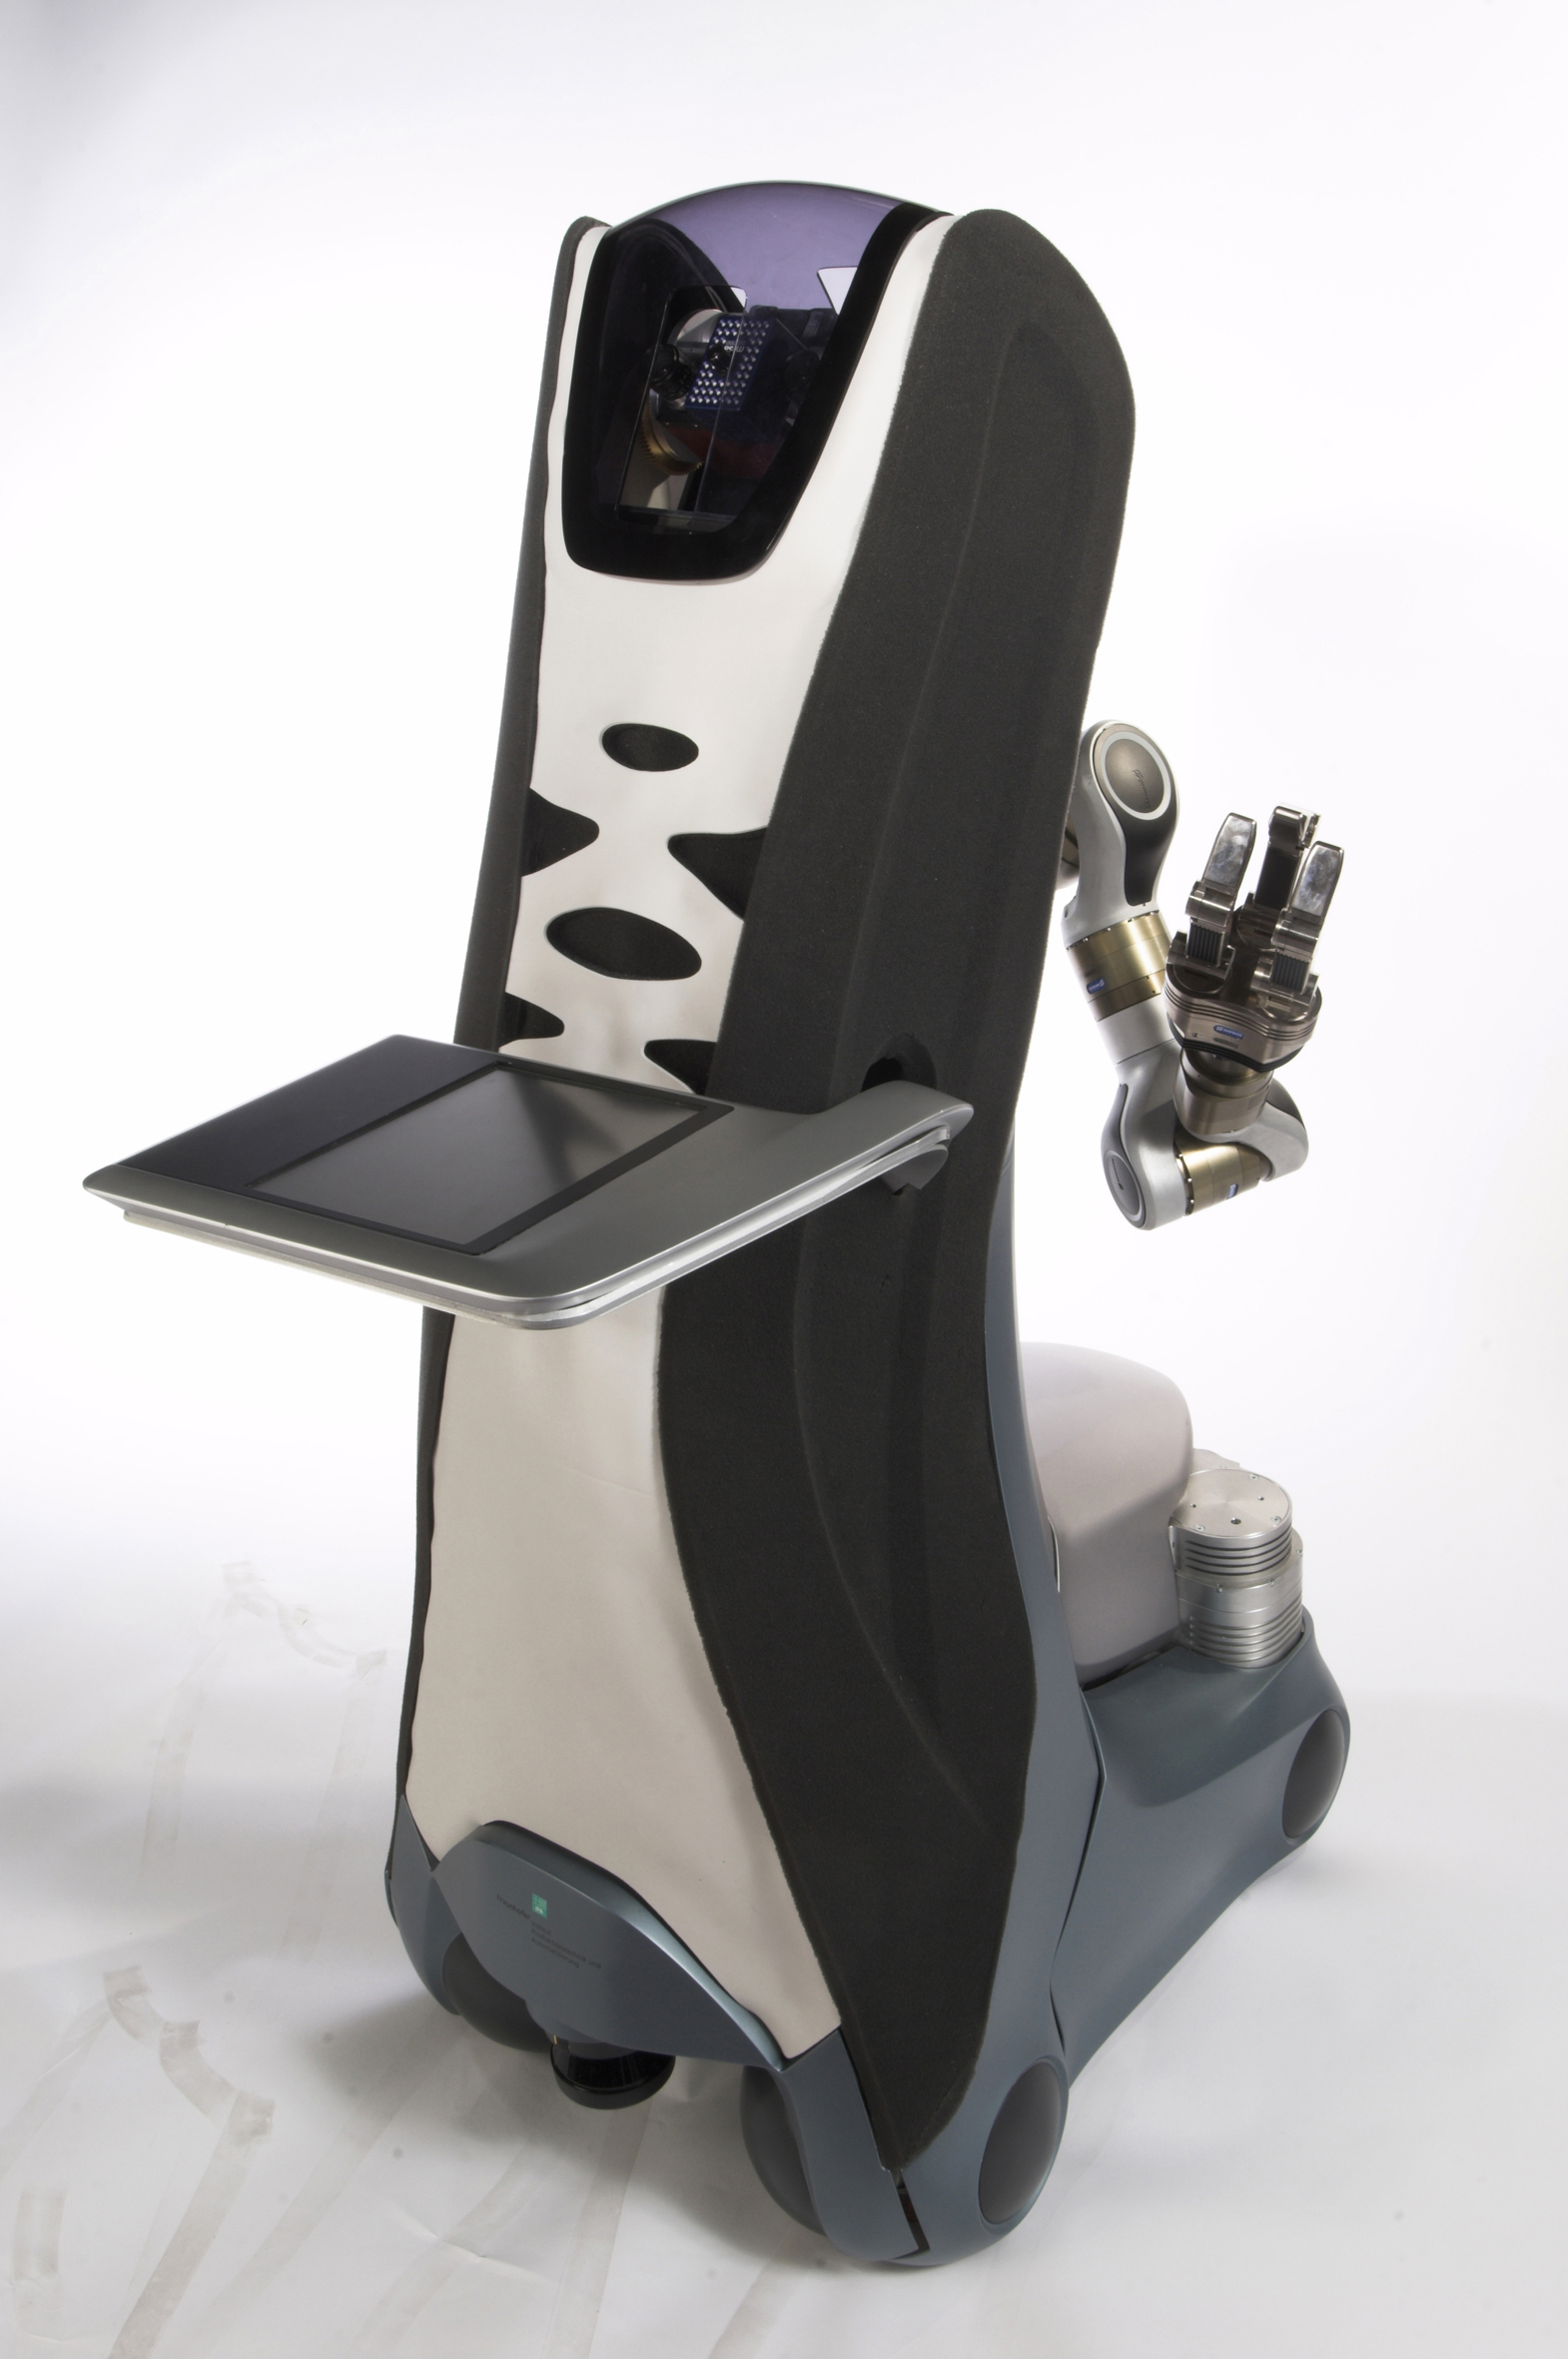
\includegraphics[width=.9\linewidth]{images/cob36}


      \end{block}

      %%%%%%%%%%%%%%%%%%%%%%%%%%%%%%%%%%%%%%%%%%%%%%%%%%%%%%%%%%%%%%%%%%%%%%%%%%%%%%%%%%%%%%%%%%%%%%%%%%%%%%%%%%%%


    \end{column}



    \begin{column}{.3\linewidth}
      %%%%%%%%%%%%%%%%%%%%%%%%%%%%%%%%%%%%%%%%%%%%%%%%%%%%%%%%%%%%%%%%%%%%%%%%%%%%%%%%%%%%%%%%%%%%%%%%%%%%%%%%%%%%
      \begin{block}{Kalibrierungsbedarf}

        CAD-Daten sind wegen dem modularen Aufbau und häufigen Änderungen nicht genau genug.
        \vskip3ex 
        \begin{itemize}
          \item Kollisionsvermeidung
          \item geplante Bewegung
          \item genaue Manipulation
        \end{itemize}
        Werden nur durch ein \alert{exaktes Modell} des \cob\ für die
        Berechnungen ermöglicht.


      \end{block}
      %%%%%%%%%%%%%%%%%%%%%%%%%%%%%%%%%%%%%%%%%%%%%%%%%%%%%%%%%%%%%%%%%%%%%%%%%%%%%%%%%%%%%%%%%%%%%%%%%%%%%%%%%%%%


      \begin{block}{Kalibrierung}

        Berechnung von Transformationen und Kameraparametern anhand von Messdaten
        eines bekannten Objekts
        \vskip1ex
        \textbf{Kalibriert werden} 
        \begin{itemize}
          \item die Montagepositionen des Arms, des Torsos und der Kameras
          \item die Kameraparameter
        \end{itemize}

        \vskip3ex
        \textbf{Bisherige Schwächen}
        \begin{itemize}
          \item nur einer von sechs \cob\ ist kalibrierbar
          \item andere nicht \cob\ sollen kalibriert werden
          \item durch mehrfache Datenaufnahme erhöhter Zeitbedarf
        \end{itemize}

        \vskip1ex
      \end{block}
      %%%%%%%%%%%%%%%%%%%%%%%%%%%%%%%%%%%%%%%%%%%%%%%%%%%%%%%%%%%%%%%%%%%%%%%%%%%%%%%%%%%%%%%%%%%%%%%%%%%%%%%%%%%%

      \begin{block}{Lösungsansätze}
        \textbf{Generalisierung} 
        \begin{itemize}
          \item Auslagern von Parametern aus dem Quellcode in 
            Konfigurationsdateien
          \item Berechnen der Positionen anhand einer neuen
            Strategie anstatt fester Karthesischer Positionen
          \item Ersetzen von zusätzlich notwendigen Denavit-Hartenberg
            Parametern durch gegebene Transformationen


        \end{itemize}

        \vskip4ex
        \textbf{Automatische Kalibrierung}
        \begin{itemize}
          \item Reduzierung auf einen Datenaufnahmeschritt
          \item Berücksichtigung des Kameramodells bei der Berechnung
        \end{itemize}
      \end{block}



    \end{column}

    %%%%%%%%%%%%%%%%%%%%%%%%%%%%%%%

    \begin{column}{.3\linewidth}

      \begin{block}{Vergleich der Kalibrierungsabläufe}
        \begin{columns}[T]
          \begin{column}{.49\linewidth}
            \begin{center}
              \textbf{\begin{large}
                Kalibrierung vorher
              \end{large}}
              \vskip4ex

              \begin{tikzpicture}[node distance = 1.5em]
                \node(positionsdaten)[rectangle split, rectangle split parts=2]
                {
                  Festgelegte 
                  \nodepart{second} Positionen für \alert{einen} Roboter\phantom{g}
                };


                \node(datenaufnahme)[rec, below = of positionsdaten]
                {
                  Datenaufnahme
                  \nodepart{second} ! Arm/ Torso Bewegung ! 
                };
                \draw[->](positionsdaten)--(datenaufnahme);

                \node (kamerakalibrierung)[comp, below=of datenaufnahme] 
                {
                  Kamerakalibrierung

                  \nodepart{second} Berechnung
                };
                \draw[->] (datenaufnahme) -- (kamerakalibrierung);


                \node (datenaufnahme2)[rec, below=of kamerakalibrierung]
                {
                  Datenaufnahme
                  \nodepart{second} ! Arm/ Torso Bewegung ! 
                };
                \draw[<-] (datenaufnahme2) -- (kamerakalibrierung);

                \node(kalibrierung) [comp, below=of datenaufnahme2] 
                {
                  kinematische Kalibrierung
                  \nodepart{second} Berechnung
                }; 
                \draw[->] (datenaufnahme2) -- (kalibrierung);

              \end{tikzpicture}
            \end{center}
          \end{column}

          \begin{column}{.49\linewidth}
            \begin{center}
              \textbf{\begin{large}
                Kalibrierung nachher
              \end{large}}
              \vskip4ex

              \begin{tikzpicture}[node distance = 1.5em]
                \node(positionsdaten)[rectangle split, rectangle split parts=2]
                {
                  Berechnete\phantom{g}  
                  \nodepart{second}Positionen für \alert{jeden} Roboter
                };


                \node(datenaufnahme)[rec, below = of positionsdaten]
                {
                  Datenaufnahme
                  \nodepart{second} ! Arm/ Torso Bewegung ! 
                };
                \draw[->](positionsdaten)--(datenaufnahme);
                \node (kamerakalibrierung)[comp, below=of datenaufnahme] 
                {
                  Kamerakalibrierung
                  \nodepart{second} Berechnung
                };
                \draw[->] (datenaufnahme) -- (kamerakalibrierung);

                \node (kalibrierung)[comp, below=of kamerakalibrierung]
                {
                  kinematische Kalibrierung 
                  \nodepart{second} Berechnung
                };
                \draw[<-] (kalibrierung) -- (kamerakalibrierung);


              \end{tikzpicture}
            \end{center}

          \end{column}
        \end{columns}
        \vskip6ex
        \textbf{Funktionen die durch die Kalibrierung ermöglicht werden}
        \begin{itemize}
          \item Objekterkennung mit den Kameras 
          \item Kollisionsvermeidung mit dem Roboter selbst
          \item Sichere Interaktion mit der Umwelt

        \end{itemize}

      \end{block}
      %%%%%%%%%%%%%%%%%%%%%%%%%%%%%%%%%%%%%%%%%%%%%%%%%%%%%%%%%%%%%%%%%%%%%%%%%%%%%%%%%%%%%%%%


      \begin{block}{Ergebnisse}
        \begin{itemize}
          \item Kalibrierung auf allen \cob\ durchführbar
          \item Kalibrierung von anderen Robotern möglich
          \item Zeit- und Sicherheitsgewinn durch einmalige Datenaufnahme
        \end{itemize}

      \end{block}

      \begin{block}{Ausblick}
        \begin{itemize}
          \item Kalibrierung der Laserscanner
          \item Kalibrierung des Tabletts
        \end{itemize}
      \end{block}

    \end{column}
  \end{columns}

\end{frame}
\end{document}


%%%%%%%%%%%%%%%%%%%%%%%%%%%%%%%%%%%%%%%%%%%%%%%%%%%%%%%%%%%%%%%%%%%%%%%%%%%%%%%%%%%%%%%%%%%%%%%%%%%%
%%% Local Variables: 
%%% mode: latex
%%% TeX-PDF-mode: t
%%% End:
